
\section{Thực hiện phần cứng (Hardware Implementation)}
\label{sec:hardware_implementation}

Hệ thống Phát hiện té ngã và Cảnh báo (FDAS) được triển khai theo kiến trúc mô-đun với hai module chính hoạt động độc lập, đảm bảo linh hoạt, khả năng giám sát rộng và duy trì hoạt động khi một module gặp sự cố. Module I tập trung vào thu thập dữ liệu chuyển động và định vị, trong khi Module II xử lý hình ảnh để xác nhận sự kiện té ngã, giảm thiểu cảnh báo sai.

\subsection{Module I: Thiết bị đeo / Cảm biến}
\label{ssec:module_one}

Module I là thiết bị phát hiện ban đầu, thiết kế nhỏ gọn để người dùng mang theo. Các thành phần chính bao gồm:

\begin{figure}[H]
    \centering
    \includegraphics[width=0.7\textwidth]{figures/module1_block_diagram-crop.pdf}
    \caption{Sơ đồ khối Module I: Thiết bị đeo / Cảm biến}
    \label{fig:module1_block_diagram}
\end{figure}

\begin{itemize}
    \item \textbf{ESP32-DevKitC-1}: Bộ vi điều khiển trung tâm, tích hợp Wi-Fi và Bluetooth, chi phí thấp, hiệu suất ổn định.
    \item \textbf{MPU6050}: Cảm biến IMU 6 trục, đo gia tốc và tốc độ góc, tích hợp bộ xử lý chuyển động DMP.
    \item \textbf{Module GPS/4G (EC800K)}: Thu thập tọa độ GPS và gửi dữ liệu cảnh báo qua mạng 4G.
    \item \textbf{Các thành phần hỗ trợ}: Buzzer và LED onboard để phản hồi tức thì khi phát hiện sự kiện.
\end{itemize}

\begin{figure}[H]
    \centering
    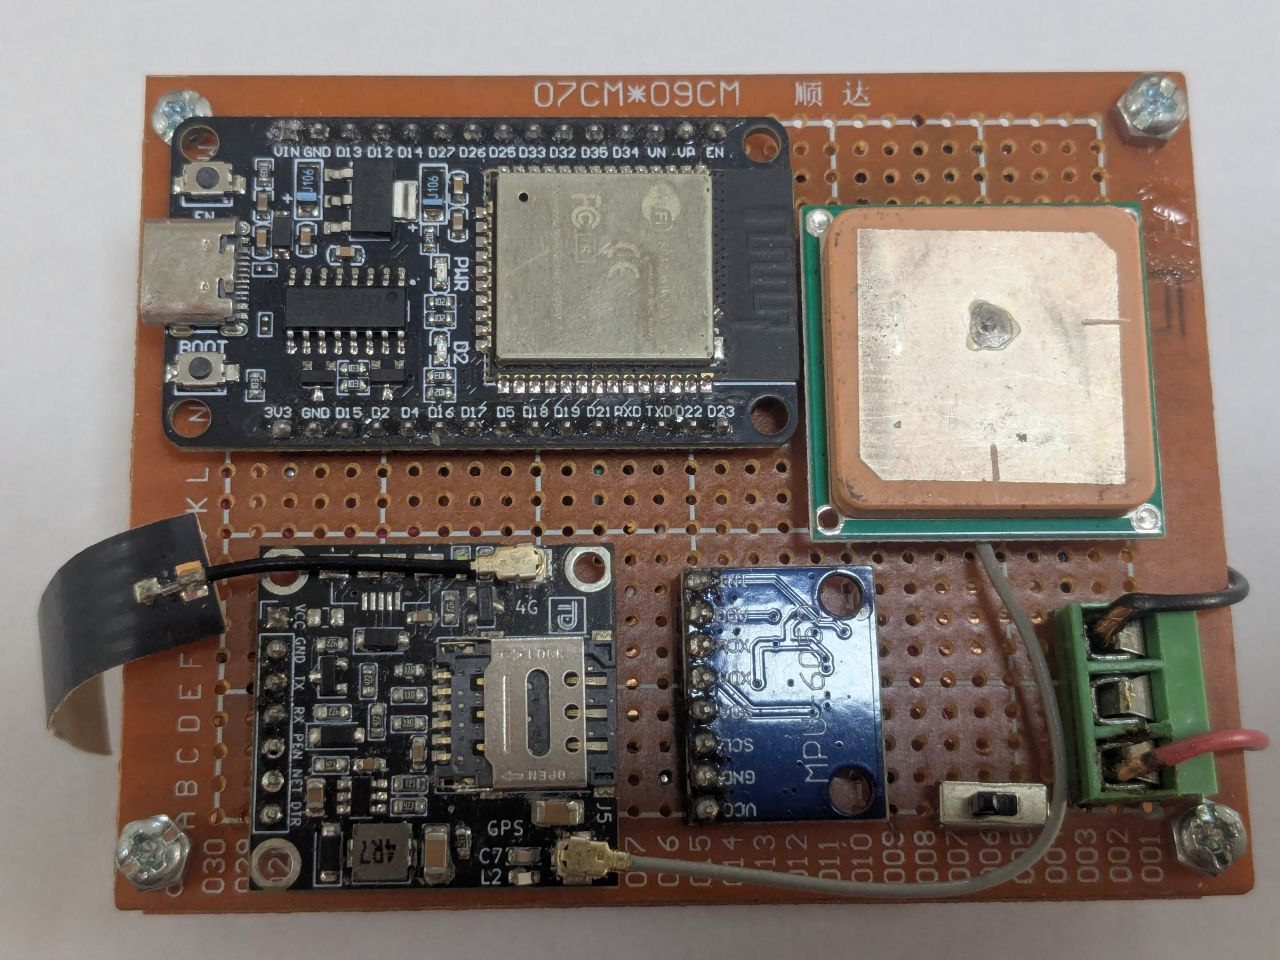
\includegraphics[width=0.8\textwidth]{figures/real_board1.jpg}
    \caption{Hình ảnh thực tế Module I đã hoàn thiện}
    \label{fig:module1_photo}
\end{figure}

Sơ đồ nguyên lý chi tiết (schematic) được vẽ bằng KiCad, đính kèm trong \textbf{Phụ lục B}.

\subsection{Module II: Camera giám sát}
\label{ssec:module_two}

Module II xác nhận sự kiện té ngã bằng hình ảnh, đặt ở khu vực giám sát trọng yếu. Các thành phần chính:

\begin{itemize}
    \item \textbf{ESP32-S3-N16R8}: Vi điều khiển mạnh mẽ, tích hợp Wi-Fi/Bluetooth, hỗ trợ PSRAM và giao diện camera chuyên dụng, tối ưu xử lý luồng dữ liệu hình ảnh.
    \item \textbf{Camera OV5640}: Cảm biến 5MP, hỗ trợ nhiều kích thước khung hình (QQVGA đến UXGA), giao tiếp dữ liệu song song 8-bit với SCCB, xung nhịp 20 MHz.
\end{itemize}

\paragraph{Sơ đồ kết nối phần cứng}
Bảng \ref{tab:pin_mapping} tóm tắt sơ đồ chân giữa ESP32-S3 và OV5640.

\begin{table}[H]
    \centering
    \caption{Sơ đồ kết nối chân giữa ESP32-S3 và OV5640}
    \label{tab:pin_mapping}
    \begin{tabular}{|l|c|l|}
    \hline
    \textbf{Chức năng} & \textbf{Chân ESP32-S3} & \textbf{Mô tả} \\
    \hline
    XCLK & 15 & Tín hiệu xung nhịp cho camera \\
    SIOD (SDA) & 4 & Dòng dữ liệu I2C \\
    SIOC (SCL) & 5 & Xung nhịp I2C \\
    D0-D7 & 11,9,8,10,12,18,17,16 & Bus dữ liệu 8-bit \\
    VSYNC & 6 & Đồng bộ khung hình dọc \\
    HREF & 7 & Tham chiếu hàng ngang \\
    PCLK & 13 & Xung nhịp điểm ảnh \\
    \hline
    \end{tabular}
\end{table}

\begin{figure}[H]
    \centering
    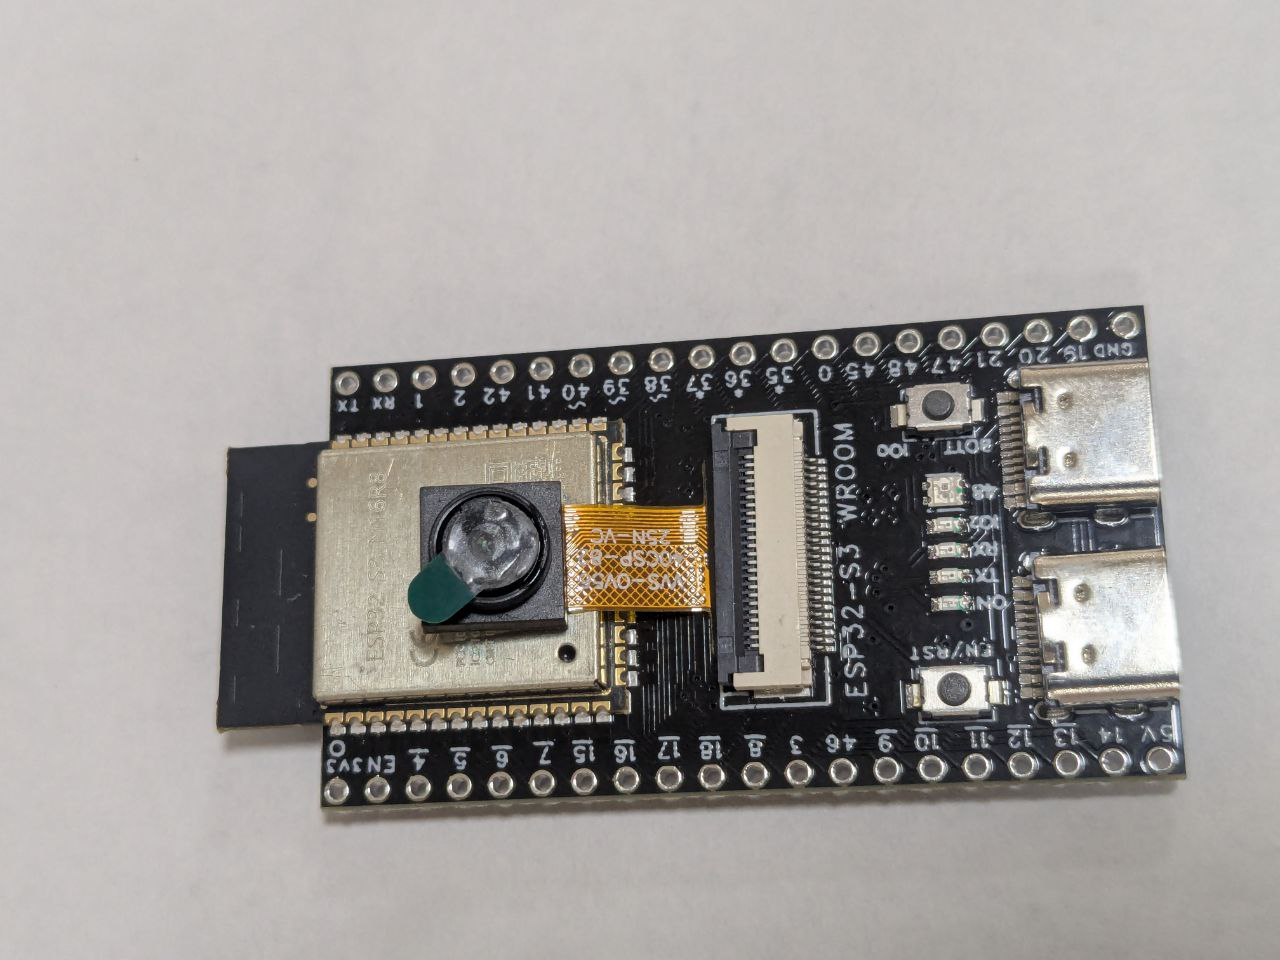
\includegraphics[width=0.8\textwidth]{figures/real_board2.jpg}
    \caption{Hình ảnh thực tế Module II}
    \label{fig:module2_photo}
\end{figure}

\subsection{Bảng tổng hợp các thành phần phần cứng}
\label{ssec:component_summary}

Bảng \ref{tab:hardware_components} tóm tắt các thành phần chính của hai module cùng vai trò và giá thành ước tính.

\begin{table}[H]
    \centering
    \caption{Tổng hợp các thành phần phần cứng}
    \label{tab:hardware_components}
    \begin{tabular}{|l|p{5cm}|p{2cm}|l|}
    \hline
    \textbf{Thành phần} & \textbf{Chức năng} & \textbf{Hình ảnh} & \textbf{Giá thành ước tính (VNĐ)} \\
    \hline
    ESP32-DevKitC-1 & Vi điều khiển chính & 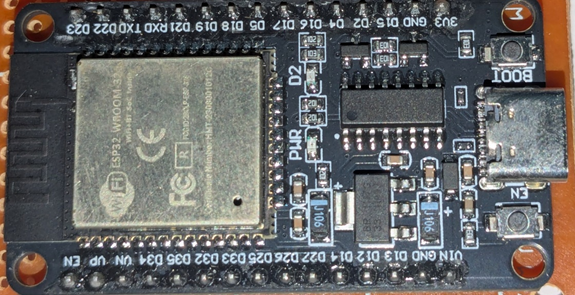
\includegraphics[width=2cm]{figures/real_esp32_c1.png} & 110.000 - 125.000 \\
    MPU6050 & Cảm biến IMU 6 trục & 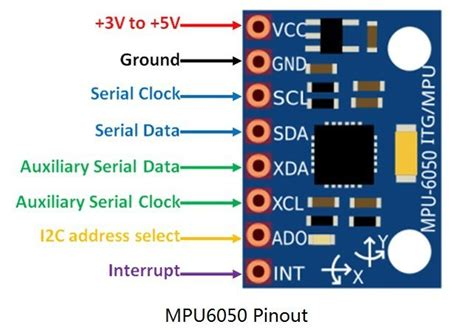
\includegraphics[width=2cm]{figures/real_mpu6050.jpg} & 45.000 - 55.000 \\
    GPS-antenna & Anten nhận GPS & 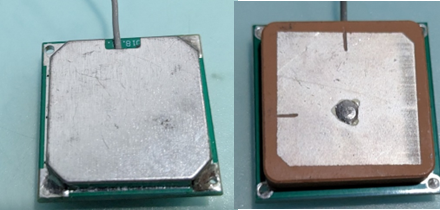
\includegraphics[width=2cm]{figures/real_gps_antenna.png} & 35.000 - 60.000 \\
    Module GPS/4G (EC800K) & Định vị và gửi cảnh báo & 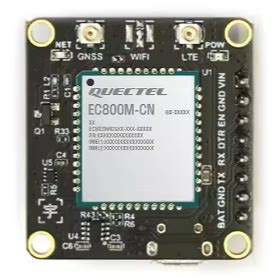
\includegraphics[width=2cm]{figures/real_ec800k.jpg} & ~240.000 \\
    Buzzer & Cảnh báo âm thanh & 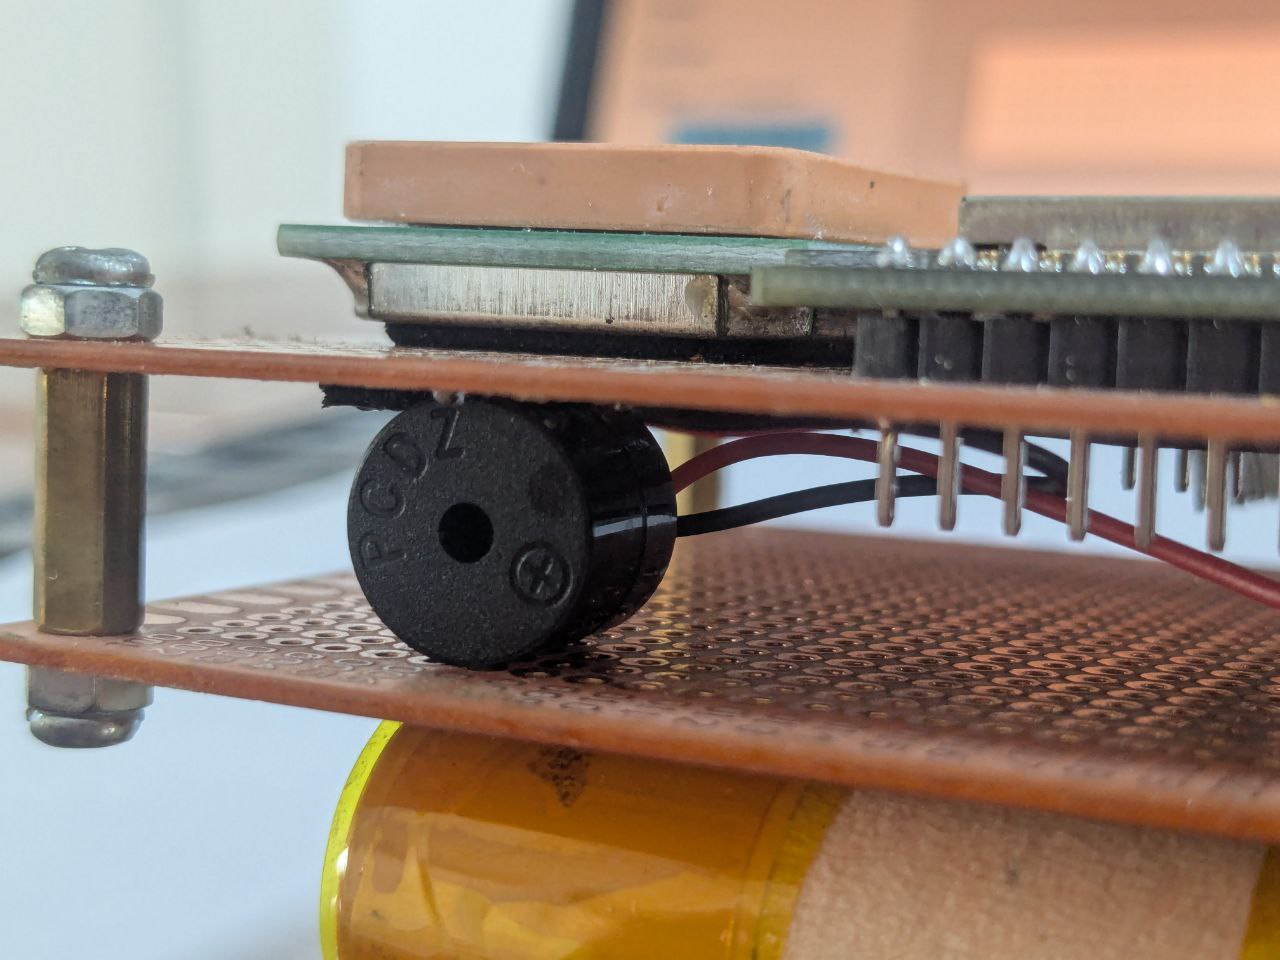
\includegraphics[width=2cm]{figures/real_buzzer.jpg} & 5.000 - 10.000 \\
    ESP32-S3-N16R8 & Vi điều khiển xử lý hình ảnh & 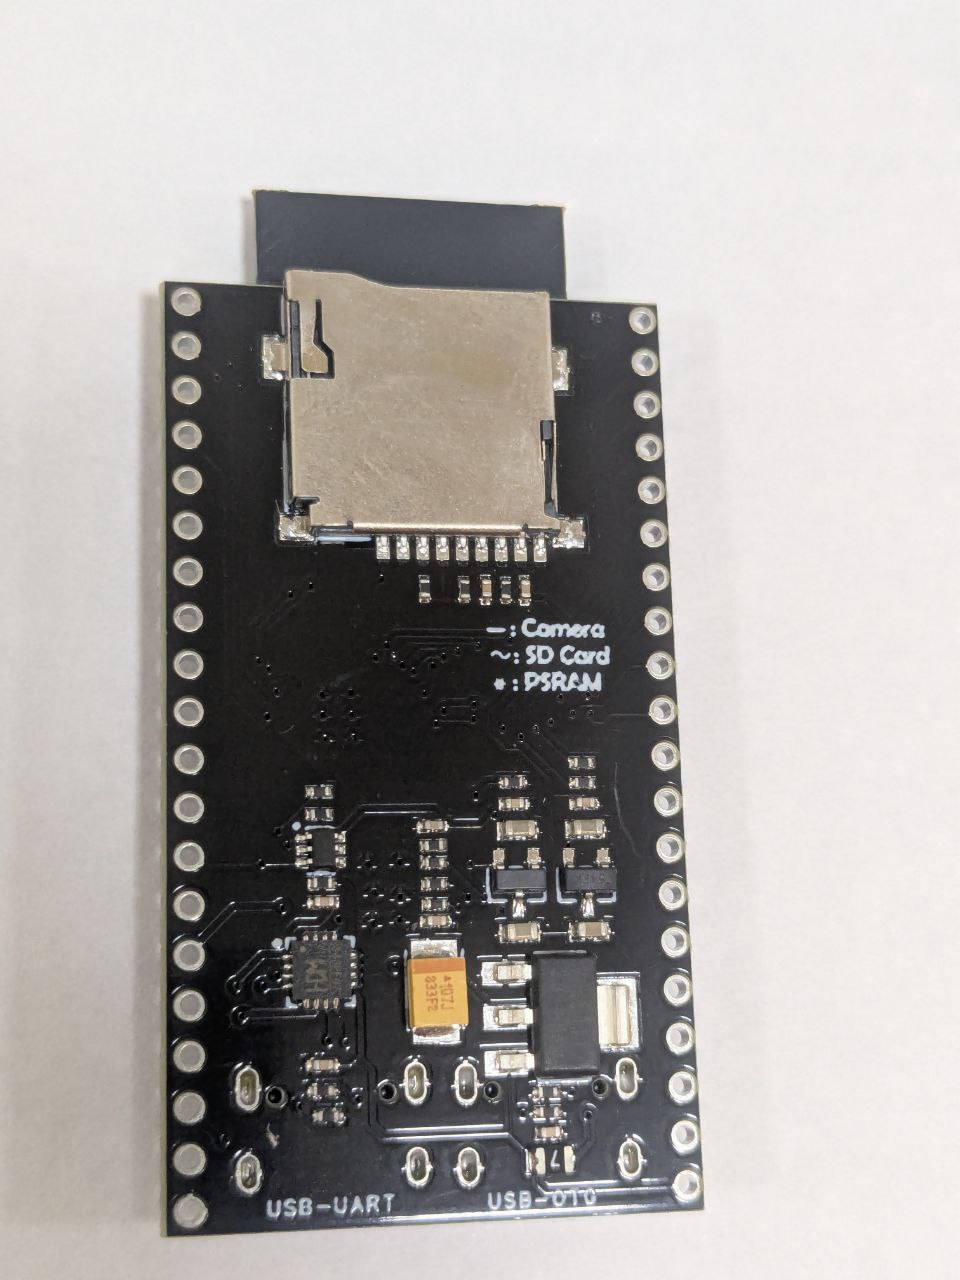
\includegraphics[width=2cm]{figures/real_esp32_s3_2.jpg} & 275.000 - 300.000 \\
    Camera OV5640 & Cảm biến hình ảnh 5MP & 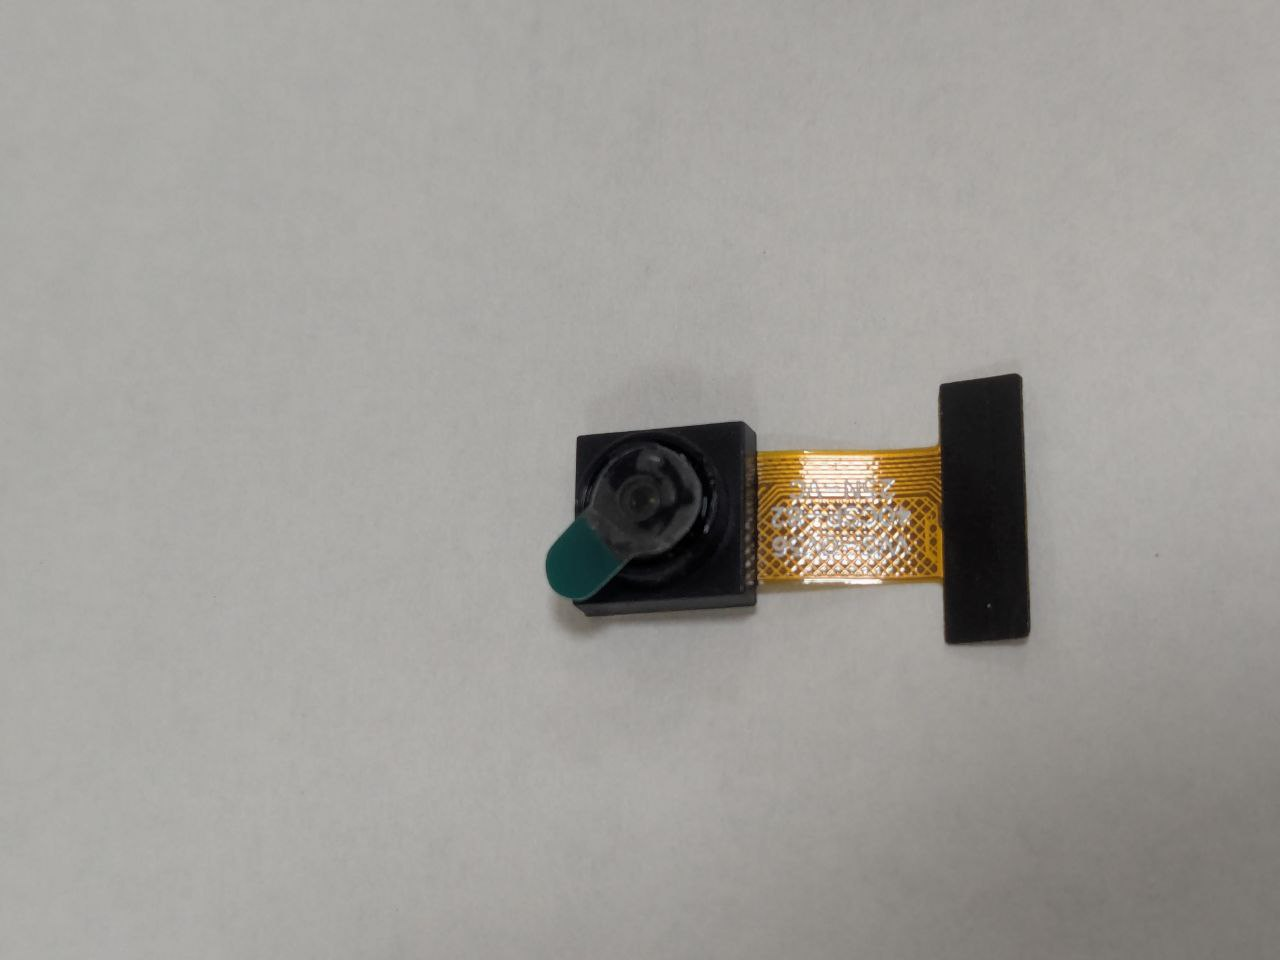
\includegraphics[width=2cm]{figures/real_ov5640.jpg} & 150.000 - 200.000 \\
    \hline
    \end{tabular}
\end{table}
